%! TEX program = xelatex

\documentclass[
    paper=A4,            % paper size --> A4 is default in Germany
    twoside=true,        % onesite or twoside printing
    openright,           % doublepage cleaning ends up right side
    parskip=full,        % spacing value / method for paragraphs
    chapterprefix=true,  % prefix for chapter marks
    12pt,                % font size
    headings=normal,     % size of headings
    bibliography=totoc,  % include bib in toc
    listof=totoc,        % include listof entries in toc
    titlepage=on,        % own page for each title page
    captions=tableabove, % display table captions above the float env
    draft=false,         % value for draft version
]{scrreprt}

\newcommand{\thesisTitle}{Thesis Title}
\newcommand{\thesisName}{Author}
\newcommand{\thesisSubject}{Documentation}
\newcommand{\thesisDate}{May 2019}
\newcommand{\thesisVersion}{First Draft}
\newcommand{\thesisUniversity}{\protect{The Chinese University of Hong Kong}}
\newcommand{\thesisUniversityDepartment}{Electronic Engineering}
\newcommand{\thesisUniversityInstitute}{Institute for Clean Thesis Dev}
\newcommand{\thesisUniversityGroup}{Clean Thesis Group (CTG)}
\newcommand{\thesisUniversityCity}{Hong Kong}
\newcommand{\thesisUniversityStreetAddress}{Rm.???, Ho Sin-hang Engineering Buidling, The Chinese University of Hong Kong, Shatin, N.T.}
\newcommand{\thesisUniversityPostalCode}{Postal Code}

% !TEX root = main.tex

\usepackage[english]{babel}
\usepackage{amsmath}
\usepackage{amsfonts}
\usepackage{bm}
\usepackage{caption}
\usepackage{graphics}
\usepackage{graphicx}
\usepackage[utf8]{inputenc}
\usepackage{lipsum}
\usepackage{multicol}
\usepackage{multirow}
\usepackage{subfigure}
\usepackage[subfigure]{tocloft}
\usepackage{url}
\usepackage[table]{xcolor}
\usepackage{xeCJK}\setCJKmainfont{Songti TC Regular}

\usepackage[
    figuresep=colon,
    sansserif=false,
    hangfigurecaption=false,
    hangsection=true,
    hangsubsection=true,
    colorize=bw,
    bibsys=biber,
    bibfile=ref,
    bibstyle=numeric,
    wrapfooter=true,
]{cleanthesis}

\hypersetup{
    pdftitle={\thesisTitle},
    pdfsubject={\thesisSubject},
    pdfauthor={\thesisName},
    plainpages=false,
    colorlinks=false,
    pdfborder={0 0 0},
    breaklinks=true,
    bookmarksnumbered=true,
    bookmarksopen=true
}

%\renewcaptionname{english}{\figurename}{Fig.}
%\renewcaptionname{english}{\tablename}{Tab.}


\begin{document}

% !TEX root = main.tex

\setstretch{1.2}
\pagenumbering{roman}
\pagestyle{empty}

\begin{titlepage}
    \pdfbookmark[0]{Titlepage}{Titlepage}
	\tgherosfont
	\centering
	\vfill
	\vspace*{1.0cm}
    {
        \addtolength{\leftskip}{-10pt}
        \addtolength{\rightskip}{-10pt}
        \LARGE \textbf{\thesisTitle} \\[30mm]
    }
	{\LARGE \thesisName } \\[30mm]
	{\Large A Thesis Submitted in Partial Fulfilment} \\[5mm]
	{\Large of the Requirements for the Degree of} \\ [5mm]
	{\Large Doctor of Philosophy} \\ [5mm]
	{\Large in } \\ [5mm]
	{\Large \thesisUniversityDepartment} \\  [40mm]
	{\Large \thesisUniversity} \\ [5mm]
 	{\Large \thesisDate}

\end{titlepage}

\cleardoublepage

% !TEX root = ../main.tex

\pagestyle{plain}

\chapter*{Abstract}
\addcontentsline{toc}{chapter}{Abstract}
\vspace*{-10mm}

\lipsum[1]

\vspace*{15mm}
\cleardoublepage

% !TEX root = ../main.tex

\newcommand{\forceindent}{\leavevmode{\parindent=1em\indent}}

\pagestyle{plain}

\chapter*{摘要}
\addcontentsline{toc}{chapter}{摘要}
\vspace*{-10mm}

\forceindent
【中大簡介】
香港中文大學(中大)成立於1963年,為研究型綜合大學,以「結合傳統與現代,融會中國與西方」為使命,蹈厲奮發,志在千里。中大師生來自世界各地。我們也有廣大的本地和海外校友組織,聯繫身在世界各地的中大畢業生。

【優質教學】
中大是香港乃至亞洲首屈一指的大學,本校的宗旨是培育既具專精知識又有處世智慧的人才,本校特色包括靈活學分制、書院制、中英兼重和多元文化;並特設通識教育 ,以拓寬學生視野,及培養綜合思考能力,使學生在瞬息萬變的現代社會中,能內省外顧,成為出色的領袖人才,貢獻社會。中大的八個學院 提供林林總總的本科 和研究院課程.

【研究稱譽】
香港中文大學研究項目包羅萬象,遍及各個學科。校方又予教員自由為業界提供顧問服務或與之協作之便。在嚴格的自我要求下,大學的研究一直保持上乘水準,享譽日隆。香港大學教育資助委員會(教資會)選定了二十四個卓越學科領域,集中資源資助本地大學進行研究,其中九個由中大學者負責。現時中文大學有五間由中國科學技術部批准成立的國家重點實驗室,具備國際一流水平的研究能力,完成國家交付的科研重任。在發表研究成果方面,中大的成績粲然可觀。無論在專門領域的學報,還是一般人耳熟能詳的期刊,如《自然》、《科學》、《刺針》,都可見中大學人的文章。

【獨有的書院制】
書院制是中大特色,在本港大學中獨一無二。現有的成員書院計有崇基學院、新亞書院、聯合書院和逸夫書院,和新增的晨興書院、善衡書院、敬文書院、伍宜孫書院及和聲書院。它們與大學相輔相成,提供以學生為本的全人教育和關顧輔導,加強師生間的交流和互動,凝聚學生對書院和母校的歸屬感。

【校園環境】
中大校園面積一百三十七點三公頃,俯瞰吐露港,是全港最寬廣、最綠意盎然的校園。為滿足學習與生活所需,校內有齊備的設施 ,包括一流的圖書館,另有文物館、音樂廳、游泳池、運動場、網球場、壁球場、水上活動中心和健身室等。

\vspace*{15mm}
\cleardoublepage

\let\forceindent\undefined

% !TEX root = ../main.tex

\chapter*{Acknowledgement}
\addcontentsline{toc}{chapter}{Acknowledgement}
\vspace*{-10mm}

\lipsum[1]

\cleardoublepage


\setstretch{1.5}
\cleardoublepage
\phantomsection
\addcontentsline{toc}{chapter}{List of Figures}
\listoffigures
\cleardoublepage
\phantomsection
\addcontentsline{toc}{chapter}{List of Tables}
\listoftables
\cleardoublepage
\phantomsection
% !TEX root = ../main.tex

\pagestyle{plain}

% acronym syntax:
% \acro{label}[acronym]{written out form}
% how to use acronyms:
% \ac = use acronym, first time write both, full name and acronym
% \acf = use full name (text + acronym)
% \acs = only use acronym
% \acl = only use long text
% \acp, acfp, acsp, aclp = use plural form for acronym (append 's')
% \acsu, aclu = write + mark as used
% \acfi = write full name in italics and acronym in normal style
% \acused = mark acronym as used
% \acfip = full, emphasized, plural, used

\chapter*{Abbreviations}
\addcontentsline{toc}{chapter}{Abbreviations}

\begin{acronym}
    \acro{NMT}[NMT]{Neural Machine Translation}
\end{acronym}

\vspace*{15mm}
\cleardoublepage


\setcounter{tocdepth}{2}
\pdfbookmark[0]{Contents}{Contents}
\tableofcontents
\cleardoublepage

\pagenumbering{arabic}
\setcounter{page}{1}
\pagestyle{maincontentstyle}

% !TEX root = main.tex

\chapter{Introduction}

Attention is all you need~\cite{vaswani2017attention}.

\begin{itemize}
    \item Item1
    \item Item2
\end{itemize}

\lipsum[1-2]

\section{Section}

\lipsum[1-2]

\begin{table}[htb]
    \centering
    \caption{Demo table}
    \begin{tabular}{c|c|c}
        cell1 & cell2 & cell3 \\ 
        \hline
        cell4 & cell5 & cell6 \\ 
        cell7 & cell8 & cell9
    \end{tabular}
\end{table}

\subsection{Subsection}

\lipsum[1-2]

\begin{figure}[htb]
\centering
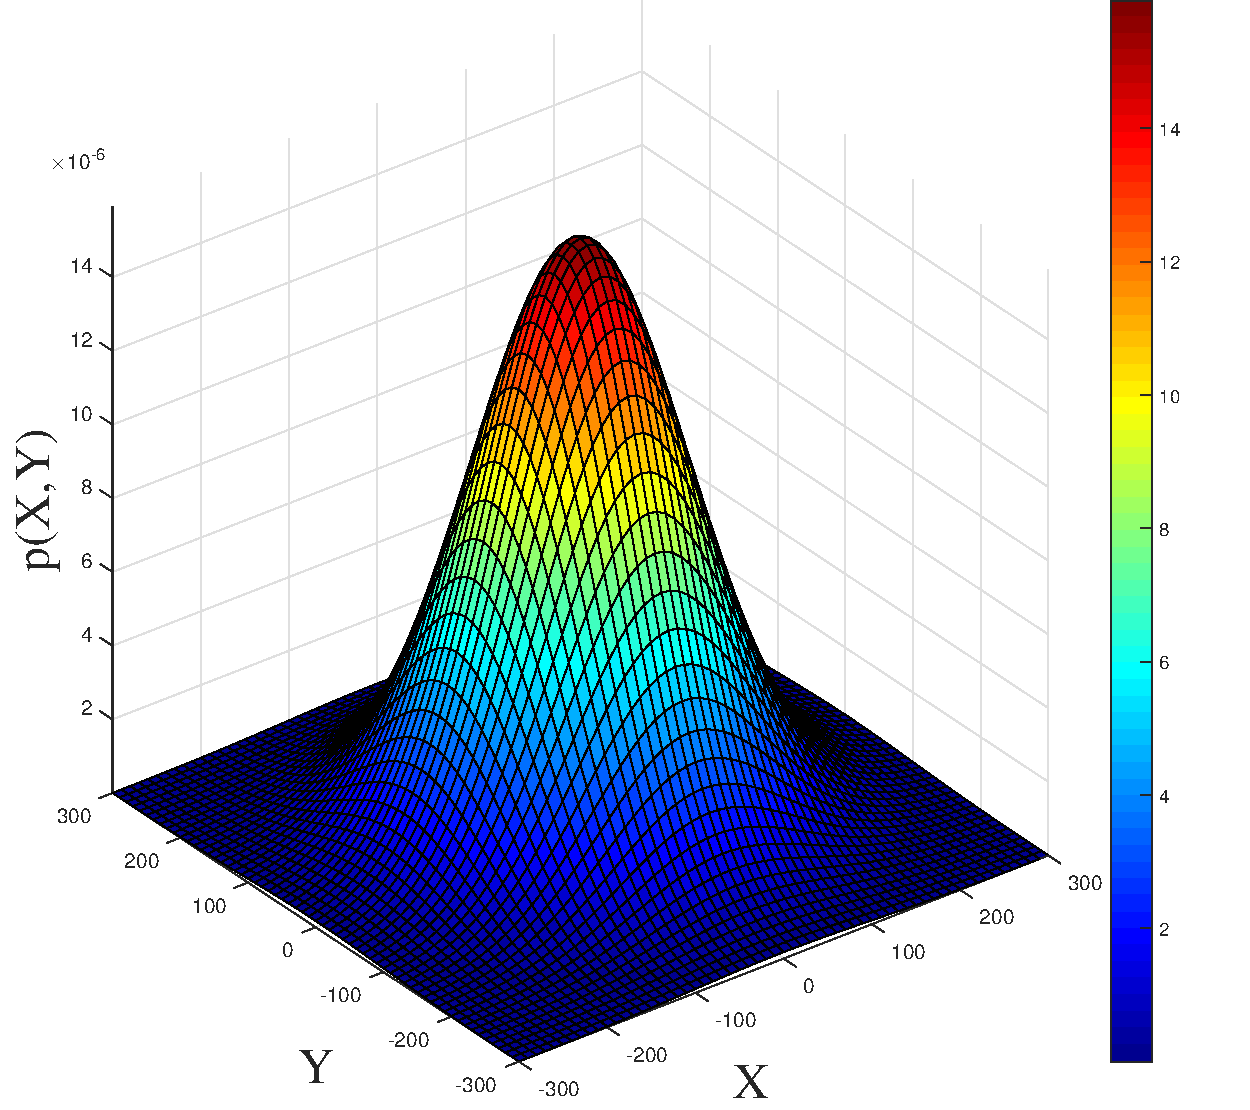
\includegraphics[width=0.5\textwidth]{fig/demo}
\caption{Demo figure}
\end{figure}

% !TEX root = ../main.tex

\chapter{Conclusions}

\lipsum[1]


\appendix
\cleardoublepage
\bibliography{ref}
\bibliographystyle{acl_natbib}
\cleardoublepage

\end{document}
